%-*- coding: UTF-8 -*-
% MathPaper.tex
%!TEX TS-program = xelatex
%!TEX encoding = UTF-8 Unicode
\documentclass[a4paper, 12pt]{article}
%设置中文字体
\usepackage{fontspec}
\setromanfont{STSongti-SC-Regular}
\XeTeXlinebreaklocale "zh"
\XeTeXlinebreakskip = 0pt plus 1pt minus 0.1pt %文章内中文自动换行

%版面设置x
\usepackage{geometry}
\geometry{left=2cm, right=2cm, top=1cm, bottom=2cm}

%首行缩进
\usepackage{indentfirst}
\setlength{\parindent}{2.45em}

%表格
\usepackage{booktabs}
%矩阵
\usepackage{amsmath}

%全局行间距
\linespread{2.1}

%去除section前面的数字
\renewcommand{\thesection}{}
\renewcommand{\thesubsection}{\arabic{section}.\arabic{subsection}}
\makeatletter
\def\@seccntformat#1{\csname #1ignore\expandafter\endcsname\csname the#1\endcsname\quad}
\let\sectionignore\@gobbletwo
\let\latex@numberline\numberline
\def\numberline#1{\if\relax#1\relax\else\latex@numberline{#1}\fi}
\makeatother

%代码
\usepackage{listings}
\usepackage{color}
\definecolor{dkgreen}{rgb}{0,0.6,0}
\definecolor{gray}{rgb}{0.5,0.5,0.5}
\definecolor{mauve}{rgb}{0.58,0,0.82}
\lstset{frame=tb,
  language=Java,
  aboveskip=3mm,
  belowskip=3mm,
  showstringspaces=false,
  columns=flexible,
  basicstyle={\small\ttfamily},
  numbers=none,
  numberstyle=\tiny\color{gray},
  keywordstyle=\color{blue},
  commentstyle=\color{dkgreen},
  stringstyle=\color{mauve},
  breaklines=true,
  breakatwhitespace=true,
  tabsize=3
}

%图片
\usepackage{graphicx}
\graphicspath{ {images/} }

\title{设计模式在iOS开发中的应用}
\author{戚海军 \\学号: MP1533024 \\Email: 2316828815@qq.com}
\date{}

\begin{document}

\maketitle

\section{}
在软件工程中,设计模式是针对特定场景下的问题的解决方案,是经时间证明为有效的,对特定面向对象设计问题的一种抽象,体现了面向对象设计的重要思想。项目如果在设计中使用了设计模式,将来就更易于复用和扩展。
在iOS开发中会使用多种设计模式,尤其是MVC模式。使用这些设计模式能使程序更加简洁而高效,达成同样目的所需的代码行会更少,更利于维护与扩展。

\newpage

\section{代理模式}
代理模式是使用一个基本上跟实体对象行为相同的代理。客户端可以透明的使用代理,不必知道所调用的只是一个代理而不是实体对象。当客户端请求某些功能时,而这些功能往往开销较大,代理将把请求转发给实体对象,准备好请求的功能并返回给客户端。客户端并不知道幕后发生了什么。代理和实体对象同样拥有客户端要求的行为。

在下列情形,会考虑使用这一模式:

需要一个远程代理,为位于不同地址空间或网络中的对象提供本地的代表。

需要一个虚拟代理,来根据要求创建重型对象。

需要一个保护代理,来根据不同访问权限控制对原对象的访问。

需要一个智能引用代理,通过对实体对象的引用进行计数来管理内存。也能用于锁定实体对象,让其他对象不能修改它。

由于Objective-C不支持多重继承,所以如果代理对象不是Cocoa Touch框架中任何类的子类的话,可以考虑使用NSProxy作为占位或代替对象。

NSProxy是Cocoa框架中的根类,如NSObject一样。NSProxy实现了NSObject协议,所以NSProxy对象实际上也是NSObject类型。NSProxy类是一个抽象基类,所以它没有自己的初始化方法。对NSProxy对象发送它不知如何响应的消息,将会抛出异常。

NSProxy的主要作用是为其他对象的替身对象定义一个API。发给代理对象的消息会被转发给实体对象,或者让代理加载实体对象,或把代理自身变成实体对象。NSProxy的子类可以用来实现创建的开销比较大的对象的懒实例化。

尽管NSproxy被看作NSObject类型,但它的存在只有一个目的,就是当代理。forwardInvocation:和methodSignatureForSelector:这两个实例方法对于整个代理过程至关重要。NSProxy的子类除了可能会需要初始化方法和几个有用的属性之外,甚至不需要其他额外的方法。关键在于,当一个NSProxy子类的对象不能响应实体对象可能会有的方法时,Objective-C的运行库会向代理对象发送一个methodSignatureForSelector:消息,取得被转发的消息的正确方法签名。接下来,运行库会使用返回的方法签名,构造一个NSInvocation实例并使用forwardInvocation:消息把它发送给代理对象,让它把调用转发给其他对象。如果作为NSProxy子类的代理对象可以响应这个消息,那么forwardInvocation:方法就根本不会被调用。
虽然Objective-C不支持多重继承,但是我们可以使用NSProxy的消息转发机制,来转发可由其他类的对象处理的任务达成同样的目的。

\newpage

\section{观察者模式}
观察者模式是定义对象间的一种一对多的依赖关系,当一个对象的状态发生改变时,所有依赖它的对象都得到通知并被自动更新。

观察者模式也叫做发布-订阅模式,它很像杂志的订阅,当从发行商订阅杂志的时候,读者把名字和邮寄地址提供给发行商,这样新的一期就能送到读者手上,发行商保证把正确的杂志送到正确的地址。一般来说读者不会收到他没有订阅的杂志,这正是观察者模式的工作方式。观察者通过通知器把自己注册到特定的通知,当有通知的时候,观察者只从通知器得到它订阅的通知。

在下列情形,会考虑使用这一模式:

有两种抽象类型相互依赖,将它们封装在各自的对象中,就可以对它们单独进行改变和复用。

对一个对象的改变需要同时改变其他对象,而不知道具体有多少对象有待改变。

一个对象必须通知其他对象,而它又不知道需要其他对象是什么。

在MVC中使用观察者模式:

MVC是一个由各种类型的设计模式组成的复合结构,观察者模式是其中的设计模式之一。View会与Controller联系在一起,等待会影响应用程序表现的事件发生。例如,当用户单击View上的“排序”按钮时,事件会传递给Controller,让Model在后台对其数据进行排序。当Model成功执行了对数据的操作后,它会通知所有相关的Controller,让它们用新的数据更新其View。

通过在MVC模式中使用观察者模式,每个组件都能够被独立复用与扩展,而对关系中的其他组件没有太多干扰。所得到的高度可复用性与可扩展性,是把其全部逻辑放入一个类中所无法获得的。因此,向Controller添加额外的View时,不用修改已有的设计和代码。同样,不同的Controller可以使用同一个Model,而不用对使用它的其他Controller作修改。尤其是Model,多个对象能够修改其内部数据。因此Model会向观察中的Controller广播特定的变更。接下来,这些Controller会命令其View用来自Model的新信息来更新其显示。

Cocoa Touch框架用两种技术改写了观察者模式——通知和键值观察。尽管是两种不同的Cocoa技术,两者都实现了观察者模式。下面将讨论他们的特征以及两者的差别。

\subsection{通知}
Cocoa Touch框架之用NSNotificationCenter和NSNotification对象实现了一对多的观察者模式。它们允许主体与观察者以一种松耦合的方式通信。两则在通信时对另一方无需多少了解。

主体要通知其他对象时,需要创建一个可通过全局的名字来识别的通知对象,然后把它投递到通知中心。通知中心查明特定通知的观察者,然后通过消息把通知发送给他们。对象订阅了特定类型的通知时,需要通过选择器提供一个方法的名字。这个方法必须符合一种单一参数的签名。方法的参数是通知对象,它包含通知名称、被观察的对象以及带有任何补充信息的字典。当有通知到来时,这个方法会被调用。

Model对象在内部数据改变之后,能够把通知投递到通知中心,使消息能够广播给其他正在观察的对象然后这些对象可做出适当的响应。Model可以像下面这样构造一个通知然后投递到通知中心:
\begin{lstlisting}
NSNotification *notification = [NSNotification notificationWithName:@"data changes" object:self];
NSNotificationCenter *notificationCenter = [NSNotificationCenter defaultCenter];
[notificationCenter postNotification:notification];
\end{lstlisting}
通知的实例可以用NSNotification类的类工厂方法,通过指定通知名和作为传给观察者的参数的任何对象来创建。在前面的例子中,通知名是“data changes”。确切的名字随时间而不同。如果主题要传递自身作为对象参数,可在创建过程中制定self来实现。

一旦创建了通知,就用它作为[notificationCenter postNotification:notification]消息调用的参数,投递到通知中心。通过向NSNotificationCenter类发送defaultcCenter消息,可以得到NSNotificationCenter实例的引用。每个进程只有一个默认的通知中心,所以默认的NSNotificationCenter是个单例对象。defaultCenter是返回应用程序中NSNotificationCenter的唯一默认实例的工厂方法。

任何要订阅这个通知的对象,首先需要为自己进行注册。如下面的代码段所示:
\begin{lstlisting}
[notificationiiCenter addObserver:self selector:@selector(update:) name:@"data changes" object:subject];
\end{lstlisting}
notificationCenter是用与主题投递通知的步骤里相同的方法得到的。要注册观察者,进行观察的对象需要在addObserver消息调用中把self注册为观察者。它也需要指定选择器,用以识别在通知中心通知这个作观察的对象时被调用的方法。对收到通知时被调用的方法,作观察的对象也可以选择设定所关心的通知的名字,以及任何其他对象作为参数。通知中心用提供的信息来确定英国想作观察的对象分发何种通知。

\subsection{键值观察}
Cocoa提供了一种称为键值观察机制,对象可以通过它得到其他对象特定属性的变更通知。这种机制在MVC模式的场景中尤其重要,因为它让View对像可以经由Controller层观察Model对象的变更。

这一机制基于NSKeyValueObserving非正式协议,Cocoa通过这个协议为所有遵守协议的对象提供了一种自动化的属性观察能力。要实现自动观察,参与键值观察的对象需要符合键值编码的要求,并且需要符合KVC的存取方法。KVC基于有关非正式协议,通过存取对象属性实现自动观察。也可以使用NSKeyValueObserving的方法和相关范畴来实现手动的观察者通知。

通知和键值观察都是Cocoa对观察者模式的改写。尽管两者都依赖观察者模式,但是它们是为不同的解决方案而设计的。
通知是一个中心对象为所有的观察者提供变更通知,主要从广义上关注程序事件。
而键值观察中被观察的对象直接向观察者发送通知,绑定于特定对象属性的值。

\newpage

\section{MVC}
MVC是iOS开发中最重要的设计模式,是Cocoa Touch中很多技术和机制的基础。在MVC设计模式中,对象在应用程序中分为3组,分别为Model、View和Controller。MVC也定义了对象之间的通信方式。如果应用程序的MVC划分的清晰,使用Cocoa Touch框架中的任何技术都会容易得多。

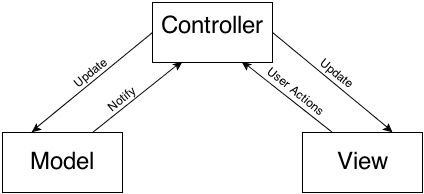
\includegraphics{mvc}

从上图中,我们可以看出Controller在MVC中起到非常重要的作用,它负责View与Model相互间的交互。当View上有了某些操作,会通过Controller反应至Model中。如果Model中的数据有所改变或者更新,则会通过Controller,对View进行相关界面改变。View与Model是永远都不直接进行通信的。

Model封装了应用程序的数据,并定义操控和处理该数据的逻辑和运算。例如,Model可能是表示游戏中的角色或地址簿中的联系人。用户在View中所进行的创建或修改数据的操作,通过Controller传达出去,最终会创建或更新Model。Model更改时(例如通过网络连接接收到新数据),它通知Controller,Controller更新相应的View。在MVC的三个部件中,Model拥有最多的处理任务。被Model返回的数据是中立的,就是说Model与数据格式无关,这样一个Model能为多个View提供数据。由于应用于Model的代码只需写一次就可以被多个View重用,所以减少了代码的重复性。

View是应用程序中用户可以看见的对象。View知道如何将自己绘制出来,并可能对用户的操作作出响应。View的主要目的,就是显示来自应用程序Model的数据,并使该数据可被编辑。尽管如此,在 MVC 应用程序中,View通常与Model分离。

在iOS应用程序开发中,所有的控件、窗口等都继承自 UIView,对应MVC中的V。UIView及其子类主要负责UI的实现,而UIView所产生的事件都可以采用委托的方式,交给UIViewController实现。

在应用程序的一个或多个View和一个或多个Model之间,Controller充当媒介。Controller因此是同步管道程序,通过它,View了解Model的更改,反之亦然。Controller还可以为应用程序执行设置和协调任务,并管理其他对象的生命周期。

Controller解释在View中进行的用户操作,并将新的或更改过的数据传达给Model。Model更改时,一个Controller会将新的Model数据传达给View,以便View可以显示它。

对于不同的UIView,有相应的UIViewController,对应MVC中的C。例如在iOS上常用的UITableView,它所对应的Controller就是UITableViewController。

Model和View永远不能相互通信,只能通过Controller传递。
Controller可以直接与Model对话,Model通过Notification和KVO机制与Controller间接通信。
Controller可以直接与View对话,通过outlet,直接操作View,outlet直接对应到View中的控件,View通过action向Controller报告事件的发生。Controller是View的直接数据源。Controller是View的代理,以同步View与Controller。

MVC的优点有很多,是Apple强烈推荐的一种设计模式:

1. 低耦合性

View层和业务层分离,这样就允许更改View层代码而不用重新编译Model和Controller代码,同样,一个应用的业务流程或者业务规则的改变只需要改动MVC的Model层即可。因为Model与Controller和View相分离,所以很容易改变应用程序的数据层和业务规则。

2. 较低的生命周期成本

MVC使开发和维护用户接口的技术含量降低。

3. 可维护性

分离View层和业务逻辑层也使得应用更易于维护和修改。

4. 有利于软件工程化管理

由于不同的层各司其职,每一层不同的应用具有某些相同的特征,有利于通过工程化、工具化管理程序代码。

\newpage

\section{单例}
单例模式保证一个类仅有一个实例,并提供一个访问它的全局访问点。要实现这一点,可以从客户端对其进行实例化开始,因此需要一种只允许生成对象类的唯一实例的机制,阻止所有想要生成对象的访问。我们可以用工厂法官法来限制实例化过程,这个方法应该是个静态方法,因为让类的实例去生成另一个唯一实例毫无意义。

在以下情形,应该考虑使用单例模式:

类只能有一个实例,而且必须从一个为人熟知的访问点对其访问,比如工厂方法;

这个唯一的实例只能通过子类化进行扩展,而且扩展的对象不会破环客户端代码。

单例模式提供了一个为人熟知的访问点,供客户端为共享资源生成唯一实例,并通过它对共享资源进行访问。虽然静态的全局对象引用或类方法也可以提供全局访问点,但是全局对象无法防止类被实例化一次以上,而且类方法也缺少消除耦合的灵活性。

静态全局变量保持者对类的实例的唯一引用,那些访问这个全局变量的类或方法,实际上是在和使用这个变量的其他类或方法共享着同一份副本。这听起来好像是我们想要的。如果在整个应用程序中都只使用同一个全局变量,那么似乎万事大吉,好像实际上并不需要单例模式,可是要是团队中的某位老兄也定义了相同类型的静态变量,那会怎么样呢?那样在同一应用程序中就会有两个相同的全局对象类型——因此全局变量并不真正解决问题。

类方法提供了共享的服务,不用创建其对象就可以访问。资源的唯一实例可在类方法中维护。然而,如果类需要被子类化以提供更好的服务,这一方式就不够灵活。

单例类提供创建和访问类的唯一对象的访问点,并保证它唯一、一致而且为人熟知。这一模式提供了灵活性,使其任何子类可以重载实例方法并且完全控制自身的对象创建,而不必修改客户端的代码。更好的是,父类中的实例实现可以处理动态对象创建。类的实际类型可以在运行时决定,以保证创建正确的对象。

单例模式有个变通版本,其中的一个工厂方法总返回同一实例,单可以分配并初始化额外的实例。

在Objective-C中实现单例模式
\begin{lstlisting}
__strong static Class *instance = nil;
static dispatch_once_t onceToken;
dispatch_once(&onceToken, ^{
	instance = [[Class alloc] init];
});
return instance;
\end{lstlisting}

\newpage

\end{document}